% ============================================================
%  SESSION 5 — React Best Practices
%  XeLaTeX ile derleyin: xelatex session-05.tex
% ============================================================
\documentclass[12pt, a4paper]{article}

% ---------- Font & Dil ----------
\usepackage{fontspec}
\usepackage[turkish, shorthands=off]{babel}
\setmainfont{Georgia}
\setsansfont{Arial}
\setmonofont{Courier New}

% ---------- Sayfa Düzeni ----------
\usepackage[top=2.2cm, bottom=2.2cm, left=2.4cm, right=2.4cm]{geometry}
\usepackage{parskip}
\setlength{\parindent}{0pt}

% ---------- Renkler ----------
\usepackage{xcolor}
\definecolor{primary}{HTML}{2563EB}
\definecolor{secondary}{HTML}{7C3AED}
\definecolor{accent}{HTML}{059669}
\definecolor{warning}{HTML}{D97706}
\definecolor{danger}{HTML}{DC2626}
\definecolor{lightbg}{HTML}{F1F5F9}
\definecolor{codebg}{HTML}{1E293B}
\definecolor{codefg}{HTML}{E2E8F0}
\definecolor{reactblue}{HTML}{61DAFB}
\definecolor{jsxcol}{HTML}{93C5FD}
\definecolor{propscol}{HTML}{FCA5A5}
\definecolor{statecol}{HTML}{86EFAC}
\definecolor{jskw}{HTML}{93C5FD}
\definecolor{jsstr}{HTML}{86EFAC}
\definecolor{jscomment}{HTML}{94A3B8}
\definecolor{hookcol}{HTML}{F59E0B}
\definecolor{refactorcol}{HTML}{EC4899}

% ---------- Kutular (tcolorbox) ----------
\usepackage[skins, breakable, listings]{tcolorbox}
\tcbuselibrary{skins, breakable, listings}

\newtcolorbox{infobox}[1][]{
  enhanced, breakable,
  colback=primary!8, colframe=primary,
  fonttitle=\bfseries\sffamily,
  title={#1},
  left=6pt, right=6pt, top=4pt, bottom=4pt,
  arc=4pt
}

\newtcolorbox{warningbox}[1][]{
  enhanced, breakable,
  colback=warning!10, colframe=warning,
  fonttitle=\bfseries\sffamily,
  title={#1},
  left=6pt, right=6pt, top=4pt, bottom=4pt,
  arc=4pt
}

\newtcolorbox{practicebox}[1][]{
  enhanced, breakable,
  colback=accent!8, colframe=accent,
  fonttitle=\bfseries\sffamily,
  title={#1},
  left=6pt, right=6pt, top=4pt, bottom=4pt,
  arc=4pt
}

\newtcolorbox{definebox}[1][]{
  enhanced, breakable,
  colback=secondary!7, colframe=secondary,
  fonttitle=\bfseries\sffamily,
  title={#1},
  left=6pt, right=6pt, top=4pt, bottom=4pt,
  arc=4pt
}

\newtcolorbox{dangerbox}[1][]{
  enhanced, breakable,
  colback=danger!7, colframe=danger,
  fonttitle=\bfseries\sffamily,
  title={#1},
  left=6pt, right=6pt, top=4pt, bottom=4pt,
  arc=4pt
}

% ---------- Kod Listeleme ----------
\usepackage{listings}

\lstset{literate=
  {ı}{{\texttt{i}}}1  {İ}{{\texttt{I}}}1
  {ğ}{{\texttt{g}}}1  {Ğ}{{\texttt{G}}}1
  {ş}{{\texttt{s}}}1  {Ş}{{\texttt{S}}}1
  {ü}{{\texttt{u}}}1  {Ü}{{\texttt{U}}}1
  {ö}{{\texttt{o}}}1  {Ö}{{\texttt{O}}}1
  {ç}{{\texttt{c}}}1  {Ç}{{\texttt{C}}}1
}

\lstdefinestyle{jsxstyle}{
  backgroundcolor=\color{codebg},
  basicstyle=\ttfamily\small\color{codefg},
  keywordstyle=\color{jskw}\bfseries,
  stringstyle=\color{jsstr},
  commentstyle=\color{jscomment}\itshape,
  morekeywords={let, const, var, async, await, of, from, import, export,
    default, class, extends, new, return, true, false, null, undefined,
    function, arrow, Promise, fetch, then, catch, finally, try,
    map, filter, reduce, forEach, find, findIndex, some, every,
    console, log, JSON, stringify, parse,
    React, useState, useEffect, useRef, useCallback, useMemo,
    props, children,
    onClick, onChange, onSubmit, onBlur, key, className, style, value,
    disabled, required, placeholder, type, htmlFor, checked,
    div, span, button, input, form, label, h1, h2, h3, p, ul, li, img,
    select, option, textarea,
    interface, type, useLocalStorage, useFetch, useToggle, useCounter,
    useDebounce, useWindowSize},
  morestring=[b]",
  morestring=[b]',
  morestring=[b]`,
  morecomment=[l]{//},
  morecomment=[s]{/*}{*/},
  showstringspaces=false,
  breaklines=true,
  frame=none,
  xleftmargin=8pt, xrightmargin=8pt,
}

% ---------- Grafikler ----------
\usepackage{graphicx}
\usepackage{caption}
\usepackage{tikz}
\usetikzlibrary{arrows.meta, shapes.geometric, positioning, calc}

% ---------- Tablo ----------
\usepackage{booktabs}
\usepackage{tabularx}
\usepackage{array}

% ---------- Başlık Stilleri ----------
\makeatletter
\renewcommand{\section}{%
  \@startsection{section}{1}{\z@}%
    {-1.5ex plus -1ex minus -0.5ex}%
    {0.8ex plus 0.3ex}%
    {\normalfont\Large\bfseries\sffamily\color{primary}}%
}
\renewcommand{\subsection}{%
  \@startsection{subsection}{2}{\z@}%
    {-1.2ex plus -0.8ex minus -0.4ex}%
    {0.5ex plus 0.2ex}%
    {\normalfont\large\bfseries\sffamily\color{secondary}}%
}
\renewcommand{\subsubsection}{%
  \@startsection{subsubsection}{3}{\z@}%
    {-1ex plus -0.6ex minus -0.3ex}%
    {0.4ex}%
    {\normalfont\normalsize\bfseries\sffamily\color{accent}}%
}
\makeatother

% ---------- Üstbilgi / Altbilgi ----------
\usepackage{fancyhdr}
\setlength{\headheight}{14pt}
\pagestyle{fancy}
\fancyhf{}
\fancyhead[L]{\small\sffamily\color{gray} Front-end + Next.js Eğitimi}
\fancyhead[R]{\small\sffamily\color{gray} Session 5 --- React Best Practices}
\fancyfoot[C]{\small\sffamily\color{gray} \thepage}
\renewcommand{\headrulewidth}{0.4pt}

% ---------- Diğer ----------
\usepackage{enumitem}
\setlist[itemize]{leftmargin=1.5em, itemsep=2pt}
\setlist[enumerate]{leftmargin=1.5em, itemsep=2pt}
\usepackage{hyperref}
\hypersetup{colorlinks=true, linkcolor=primary, urlcolor=primary}
\usepackage{fontawesome5}

% ---------- Yardımcı Komut ----------
\newcommand{\timebadge}[1]{%
  \noindent
  \colorbox{primary}{\color{white}\sffamily\bfseries\small\strut~~\faStopwatch~~#1~~}%
  \par\vspace{4pt}%
}

\newcommand{\jsinline}[1]{\texttt{\color{primary}#1}}

% ============================================================
\begin{document}

% ============================================================
%  KAPAK
% ============================================================
\thispagestyle{empty}

\begin{tikzpicture}[remember picture, overlay]
  \fill[primary] (current page.north west)
    rectangle ++(\paperwidth, -8.0cm);
  \fill[secondary] (current page.north west) ++(0,-7.8cm)
    rectangle ++(\paperwidth, -0.28cm);
\end{tikzpicture}

\vspace*{1.6cm}
{\color{white}\sffamily
  \hspace{1.2cm}{\small SESSION 5 / 8 \quad|\quad 7 Mayıs 2026 \quad|\quad~90 dakika}\\[12pt]
  \hspace{1.2cm}{\fontsize{30}{36}\selectfont\bfseries React Best Practices}\\[8pt]
  \hspace{1.2cm}{\Large Component Parçalama, State Yönetimi, Custom Hooks}
}

\vspace{0.9cm}

\vspace{0.1cm}

\begin{tcolorbox}[enhanced,
  colback=lightbg, colframe=gray!30, arc=4pt,
  title={\sffamily\bfseries\color{primary}\faStream\quad Session Akışı},
  fonttitle=\bfseries\sffamily]
\sffamily\small
\begin{tabularx}{\textwidth}{>{\bfseries\color{primary}}l X l}
\toprule
Süre & Konu & Anahtar Kavramlar \\
\midrule
0--25 dk  & Component Parçalama                & SRP, reusable component, prop drilling \\
25--45 dk & State Yönetimi Yaklaşımı           & lifting state up, prop drilling \\
45--65 dk & Custom Hooks                       & use* prefix, mantık paylaşımı \\
65--90 dk & \textcolor{accent}{Pratik: ToDo Refactor} & component split + custom hook \\
\bottomrule
\end{tabularx}
\end{tcolorbox}

% ============================================================
\clearpage
\section{\faPuzzlePiece\ Component Parçalama}
\timebadge{0--25 dakika}

\subsection{Neden Component Parçalamalıyız?}

Session 4'te yazdığımız ToDo uygulaması tek bir \texttt{TodoApp}
component'inde 100+ satır kod barındırıyordu. Bu yaklaşım küçük projelerde
çalışır ama uygulama büyüdükçe sorunlar başlar:

\begin{itemize}
  \item Kod okunması zorlaşır --- her şey aynı dosyada
  \item Aynı UI parçası birkaç yerde lazım olunca kopyalanır
  \item Hata ayıklamak zorlaşır --- nerede hata var?
  \item Test yazmak zor olur
  \item Birden fazla geliştirici aynı dosyada çalışınca çakışmalar artar
\end{itemize}

\vspace{6pt}

\begin{definebox}[Single Responsibility Principle (SRP)]
Her component \textbf{tek bir iş} yapmalıdır. Bir component
``hem listeyi göster, hem de ekleme formunu yönet, hem de validation yap''
demek yerine; \textbf{her sorumluluk ayrı bir component} olmalıdır.
\end{definebox}

% ----------------------------------------------------------
\subsection{Önce / Sonra Karşılaştırması}

\subsubsection{Önce --- Tek Büyük Component}

\begin{tcolorbox}[enhanced, colback=codebg, colframe=gray!30,
    colbacktitle=danger!85!black, coltitle=white, arc=4pt,
    title={\sffamily\bfseries\small \faTimes\ TodoApp.tsx --- Her şey tek dosyada}]
\begin{lstlisting}[style=jsxstyle]
function TodoApp() {
  const [todos, setTodos] = useState([]);
  const [text, setText] = useState("");

  // ... ekleme, silme, toggle fonksiyonlari ...

  return (
    <div>
      <h1>Todos</h1>

      {/* Form --- 20 satir kod */}
      <form onSubmit={handleAdd}>
        <input value={text} onChange={...} />
        <button type="submit">Add</button>
      </form>

      {/* Liste --- 30 satir kod */}
      <ul>
        {todos.map(todo => (
          <li key={todo.id}>
            <input type="checkbox" .../>
            <span>{todo.text}</span>
            <button onClick={...}>Delete</button>
          </li>
        ))}
      </ul>

      {/* Ozet --- 10 satir kod */}
      <p>{remaining} remaining</p>
    </div>
  );
}
\end{lstlisting}
\end{tcolorbox}

\vspace{6pt}

\subsubsection{Sonra --- Parçalanmış Component'ler}

\begin{tcolorbox}[enhanced, colback=codebg, colframe=gray!30,
    colbacktitle=accent!85!black, coltitle=white, arc=4pt,
    title={\sffamily\bfseries\small \faCheck\ TodoApp.tsx --- Sadece koordinasyon}]
\begin{lstlisting}[style=jsxstyle]
function TodoApp() {
  const [todos, setTodos] = useState([]);

  const addTodo = (text) => { /* ... */ };
  const toggleTodo = (id) => { /* ... */ };
  const deleteTodo = (id) => { /* ... */ };

  return (
    <div>
      <h1>Todos</h1>
      <TodoForm onAdd={addTodo} />
      <TodoList
        todos={todos}
        onToggle={toggleTodo}
        onDelete={deleteTodo}
      />
      <TodoStats todos={todos} />
    </div>
  );
}
\end{lstlisting}
\end{tcolorbox}

\vspace{6pt}

\begin{center}
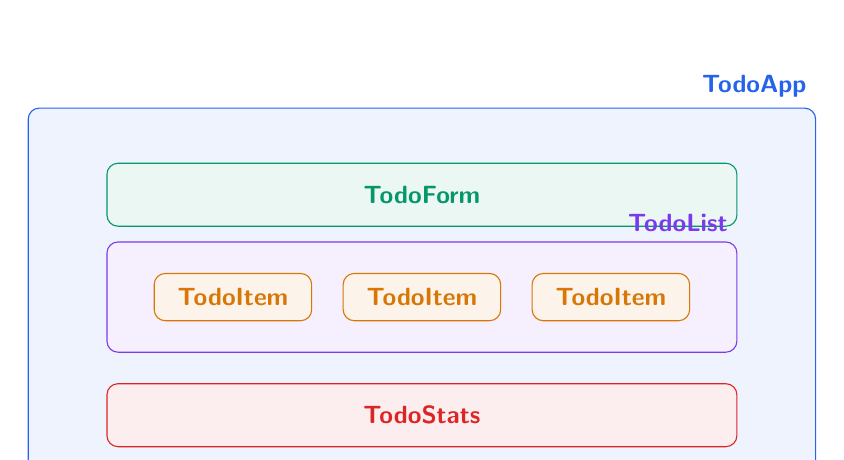
\begin{tikzpicture}[
  box/.style={draw=#1, fill=#1!8, rounded corners=4pt,
    minimum height=0.9cm, font=\sffamily\small\bfseries, text=#1},
  >=Stealth
]
  \node[box=primary, minimum width=10cm, minimum height=4.6cm] (app) at (0,0) {};
  \node[primary, font=\sffamily\bfseries\small, above left] at (app.north east) {TodoApp};

  \node[box=accent, minimum width=8cm, minimum height=0.8cm]
    (form) at (0, 1.2) {TodoForm};

  \node[box=secondary, minimum width=8cm, minimum height=1.4cm]
    (list) at (0, -0.1) {};
  \node[secondary, font=\sffamily\bfseries\small, above left] at (list.north east) {TodoList};

  \node[box=warning, minimum width=2.0cm, minimum height=0.6cm]
    (item1) at (-2.4,-0.1) {TodoItem};
  \node[box=warning, minimum width=2.0cm, minimum height=0.6cm]
    (item2) at (0,-0.1)    {TodoItem};
  \node[box=warning, minimum width=2.0cm, minimum height=0.6cm]
    (item3) at (2.4,-0.1)  {TodoItem};

  \node[box=danger, minimum width=8cm, minimum height=0.8cm]
    (stats) at (0, -1.6) {TodoStats};
\end{tikzpicture}
\end{center}

% ----------------------------------------------------------
\newpage
\subsection{Component Parçalama Sinyalleri}

Bir component'i ne zaman parçalamalıyım? Aşağıdaki sinyalleri arayın:

\vspace{6pt}

\begin{tcolorbox}[enhanced, colback=lightbg, colframe=gray!30, arc=4pt]
\sffamily\small
\begin{tabularx}{\textwidth}{>{\bfseries\color{primary}}l X}
\toprule
Sinyal & Açıklama \\
\midrule
Çok uzun JSX &
  100+ satır return bloğu varsa parçalama zamanı geldi. \\[4pt]
Tekrarlayan yapı &
  Aynı JSX bloğu \texttt{map} dışında 2+ yerde varsa component yap. \\[4pt]
Anlaşılması zor isim &
  ``Bu \texttt{<div>} ne işe yarıyor?'' diye düşünüyorsanız ona isim verin. \\[4pt]
Bağımsız davranış &
  Bir bölüm kendi state/effect'ini yönetiyorsa ayrı component olabilir. \\[4pt]
Yeniden kullanım &
  Aynı UI başka bir sayfada da lazım olacaksa component yapın. \\
\bottomrule
\end{tabularx}
\end{tcolorbox}

\vspace{6pt}

\begin{infobox}[\faLightbulb\ Sezgisel Kural]
Bir component'i \textbf{üst üste 2--3 ekran kaydırarak} okumak zorunda
kalıyorsanız, parçalama vakti gelmiş demektir.
``Ne yapıyor?'' sorusuna tek cümlede cevap veremiyorsanız da öyle.
\end{infobox}

% ----------------------------------------------------------
\subsection{Reusable (Yeniden Kullanılabilir) Component}

Reusable component, farklı yerlerde \textbf{farklı veriyle} aynı görünümü
sağlayabilen component'tir. Anahtar nokta: davranış props ile dışarıdan
kontrol edilir.

\vspace{6pt}

\subsubsection{Kötü --- Sabit Veriye Bağımlı}

\begin{tcolorbox}[enhanced, colback=codebg, colframe=gray!30,
    colbacktitle=danger!85!black, coltitle=white, arc=4pt,
    title={\sffamily\bfseries\small \faTimes\ Yeniden kullanılamaz}]
\begin{lstlisting}[style=jsxstyle]
function PrimaryButton() {
  return (
    <button
      onClick={() => alert("Saved!")}
      style={{ background: "#2563eb", color: "white" }}
    >
      Save
    </button>
  );
}
\end{lstlisting}
\end{tcolorbox}

\vspace{4pt}

\begin{dangerbox}[\faExclamationCircle\ Sorun]
Bu buton sadece ``Save'' yazısı için, sadece alert için, sadece mavi renk için
çalışır. Başka yerde kullanmak için kopyala-yapıştır yapmanız gerekir.
\end{dangerbox}

\vspace{6pt}

\subsubsection{İyi --- Props ile Esnek}

\begin{tcolorbox}[enhanced, colback=codebg, colframe=gray!30,
    colbacktitle=accent!85!black, coltitle=white, arc=4pt,
    title={\sffamily\bfseries\small \faCheck\ Reusable Button}]
\begin{lstlisting}[style=jsxstyle]
interface ButtonProps {
  children: React.ReactNode;
  onClick?: () => void;
  variant?: "primary" | "danger" | "ghost";
  disabled?: boolean;
}

function Button({
  children,
  onClick,
  variant = "primary",
  disabled = false,
}: ButtonProps) {
  const colors = {
    primary: { bg: "#2563eb", fg: "white" },
    danger:  { bg: "#ef4444", fg: "white" },
    ghost:   { bg: "transparent", fg: "#2563eb" },
  };
  const c = colors[variant];

  return (
    <button
      onClick={onClick}
      disabled={disabled}
      style={{
        background: c.bg, color: c.fg,
        padding: "10px 20px", border: "none",
        borderRadius: 8, cursor: "pointer",
        opacity: disabled ? 0.5 : 1,
      }}
    >
      {children}
    </button>
  );
}

// Kullanim --- ayni component, farkli amaclar
<Button onClick={save}>Save</Button>
<Button variant="danger" onClick={remove}>Delete</Button>
<Button variant="ghost" onClick={cancel}>Cancel</Button>
\end{lstlisting}
\end{tcolorbox}

\vspace{6pt}

\begin{infobox}[\faLightbulb\ Reusable Component Tarifi]
\begin{enumerate}
  \item İçeriği \texttt{children} prop'undan al
  \item Davranışı (\texttt{onClick}, \texttt{onChange}\ldots) prop'tan al
  \item Görünümü \texttt{variant}, \texttt{size} gibi prop'larla yönet
  \item Default değerleri tanımla (\texttt{variant = "primary"})
  \item Component \textbf{ne göstereceğini} bilmesin --- sadece \textbf{nasıl
        görüneceğini} bilsin
\end{enumerate}
\end{infobox}

% ============================================================
\newpage
\section{\faProjectDiagram\ State Yönetimi Yaklaşımı}
\timebadge{25--45 dakika}

\subsection{State Nerede Yaşamalı?}

Component'leri parçaladıkça yeni bir soru çıkar: \textbf{state'i nereye koyalım?}

\vspace{6pt}

\begin{definebox}[Lifting State Up (Hatırlama)]
Birden fazla component'in \textbf{aynı veriye} ihtiyacı varsa,
o veri (state) onların \textbf{ortak ata}sında (parent) tutulmalıdır.
Aşağıya \textbf{props}, yukarıya \textbf{callback} ile akar.
\end{definebox}

\vspace{6pt}

\begin{center}
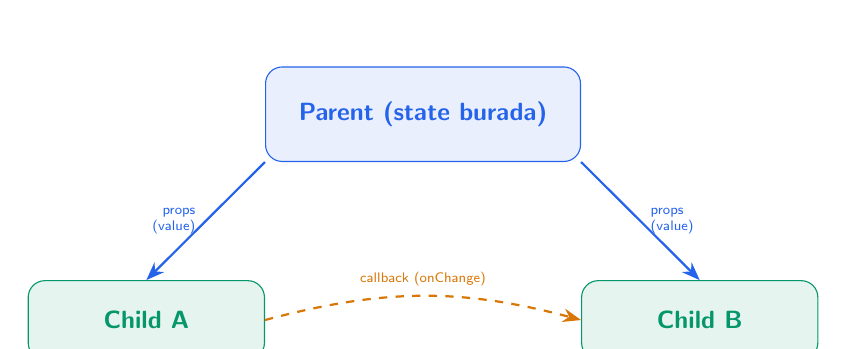
\begin{tikzpicture}[>=Stealth]
  \node[draw=primary, fill=primary!10, rounded corners=6pt,
        minimum width=4.0cm, minimum height=1.2cm,
        font=\sffamily\bfseries\small, text=primary] (parent)
        {Parent (state burada)};

  \node[draw=accent, fill=accent!10, rounded corners=6pt,
        minimum width=3.0cm, minimum height=1.0cm,
        font=\sffamily\bfseries\small, text=accent,
        below left=1.5cm and 0.0cm of parent] (childA)
        {Child A};

  \node[draw=accent, fill=accent!10, rounded corners=6pt,
        minimum width=3.0cm, minimum height=1.0cm,
        font=\sffamily\bfseries\small, text=accent,
        below right=1.5cm and 0.0cm of parent] (childB)
        {Child B};

  \draw[->, thick, primary]
    (parent.south west) -- node[left, font=\sffamily\tiny, text=primary, align=right]
    {props\\(value)} (childA.north);

  \draw[->, thick, primary]
    (parent.south east) -- node[right, font=\sffamily\tiny, text=primary, align=left]
    {props\\(value)} (childB.north);

  \draw[->, thick, warning, dashed]
    (childA.east) to[bend left=15]
    node[above, font=\sffamily\tiny, text=warning] {callback (onChange)}
    (childB.west);

\end{tikzpicture}
\end{center}

\vspace{6pt}

\subsubsection{Lifting State Up Örneği}

İki sıcaklık inputu (Celsius ve Fahrenheit), ikisi de aynı sıcaklığı temsil
ediyor. State'i ortak ata olan \texttt{TemperatureCalculator}'a taşırız:

\begin{tcolorbox}[enhanced, colback=codebg, colframe=gray!30,
    colbacktitle=primary!85!black, coltitle=white, arc=4pt,
    title={\sffamily\bfseries\small Lifting State Up}]
\begin{lstlisting}[style=jsxstyle]
function TemperatureCalculator() {
  // State, hem Celsius hem Fahrenheit input'unun ihtiyaci olan veridir.
  // Bu yuzden ortak parent'a koyduk.
  const [celsius, setCelsius] = useState(0);
  const fahrenheit = celsius * 9 / 5 + 32;

  return (
    <div>
      <CelsiusInput
        value={celsius}
        onChange={setCelsius}
      />
      <FahrenheitInput
        value={fahrenheit}
        onChange={(f) => setCelsius((f - 32) * 5 / 9)}
      />
    </div>
  );
}

function CelsiusInput({ value, onChange }) {
  return (
    <label>
      Celsius:
      <input
        type="number"
        value={value}
        onChange={(e) => onChange(Number(e.target.value))}
      />
    </label>
  );
}

function FahrenheitInput({ value, onChange }) {
  return (
    <label>
      Fahrenheit:
      <input
        type="number"
        value={value}
        onChange={(e) => onChange(Number(e.target.value))}
      />
    </label>
  );
}
\end{lstlisting}
\end{tcolorbox}

% ----------------------------------------------------------
\newpage
\subsection{Props Drilling --- ve Sınırı}

\begin{definebox}[Props Drilling]
State'i kullanmak için onu \textbf{birkaç katman aşağıdaki} component'e
taşımak gerekiyorsa, aradaki tüm component'lere prop olarak geçirmek
zorundayız. Buna \textbf{props drilling} denir.
\end{definebox}

\vspace{8pt}

\begin{center}
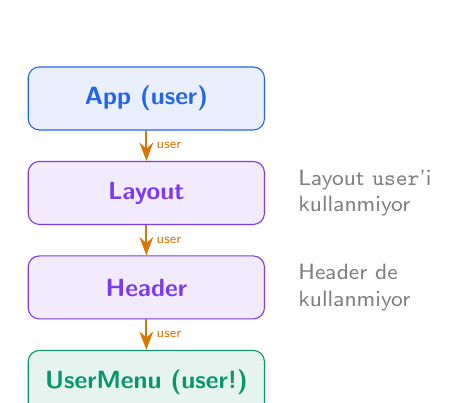
\begin{tikzpicture}[
  box/.style={draw=#1, fill=#1!10, rounded corners=4pt,
    minimum width=3.0cm, minimum height=0.8cm,
    font=\sffamily\small\bfseries, text=#1},
  >=Stealth
]
  \node[box=primary] (a) at (0, 3.6) {App (user)};
  \node[box=secondary] (b) at (0, 2.4) {Layout};
  \node[box=secondary] (c) at (0, 1.2) {Header};
  \node[box=accent]    (d) at (0, 0.0) {UserMenu (user!)};

  \draw[->, thick, warning] (a.south) -- node[right, font=\sffamily\tiny, text=warning] {user} (b.north);
  \draw[->, thick, warning] (b.south) -- node[right, font=\sffamily\tiny, text=warning] {user} (c.north);
  \draw[->, thick, warning] (c.south) -- node[right, font=\sffamily\tiny, text=warning] {user} (d.north);

  \node[font=\sffamily\footnotesize, text=gray, right=0.3cm of b, align=left]
    {Layout \texttt{user}'i\\kullanmiyor};
  \node[font=\sffamily\footnotesize, text=gray, right=0.3cm of c, align=left]
    {Header de\\kullanmiyor};
\end{tikzpicture}
\end{center}

\vspace{6pt}

\begin{warningbox}[\faExclamationTriangle\ Props Drilling Ne Zaman Sorun?]
\begin{itemize}
  \item Ara katmanlar veriyi \textbf{sadece geçirmek için} alıyorsa
  \item 3+ katman derinliğinde aynı prop dolaşıyorsa
  \item Yeni bir prop eklerken \textbf{birçok dosyayı düzenlemek} gerekiyorsa
\end{itemize}
\end{warningbox}

\vspace{6pt}

\begin{infobox}[\faLightbulb\ Çözüm Hiyerarşisi]
\begin{enumerate}
  \item \textbf{Önce}: 1--2 katman ise sorun değil, bırakın --- en basit çözüm.
  \item \textbf{Component composition}: \texttt{children} ile veriyi
        ara katmanlardan geçirmemek mümkün.
  \item \textbf{React Context}: Tema, dil, kullanıcı gibi global veriler için.
  \item \textbf{State management kütüphaneleri}: Redux, Zustand, Jotai
        --- karmaşık uygulamalar için (bu kursta detaya girmiyoruz).
\end{enumerate}
\end{infobox}

% ----------------------------------------------------------
\subsection{State Yönetiminde Kararlar}

\begin{tcolorbox}[enhanced, colback=lightbg, colframe=gray!30, arc=4pt]
\sffamily\small
\begin{tabularx}{\textwidth}{>{\bfseries\color{primary}}l X}
\toprule
Soru & Cevap \\
\midrule
Tek component kullanıyor mu? & Lokal \texttt{useState} \\[4pt]
İki kardeş component kullanıyor mu? & Ortak parent'a kaldır (lifting up) \\[4pt]
Çok derinde sadece bir yerde lazım mı? & Component composition (\texttt{children}) \\[4pt]
Birçok yerde global lazım mı? & React Context veya state lib \\[4pt]
Sunucudan gelen veri mi? & Server state lib (TanStack Query --- ileride) \\
\bottomrule
\end{tabularx}
\end{tcolorbox}

\vspace{6pt}

\begin{definebox}[Altın Kural]
Önce \textbf{en yakın ortak parent}'ı seç. Çok kalabalık olursa parçala.
Daha gelişmiş çözümleri sadece \textbf{ihtiyaç} duyduğunda getir.
\end{definebox}

% ============================================================
\newpage
\section{\faMagic\ Custom Hooks}
\timebadge{45--65 dakika}

\subsection{Custom Hook Nedir?}

\begin{definebox}[Custom Hook]
Custom hook, \textbf{ismi \texttt{use} ile başlayan} ve içinde diğer
hook'ları (\texttt{useState}, \texttt{useEffect}\ldots) çağıran bir
\textbf{JavaScript fonksiyonudur}. Component değildir, JSX döndürmez ---
\textbf{state mantığını} döndürür.
\end{definebox}

\vspace{6pt}

\subsubsection{Neden Custom Hook?}

Birden fazla component'te aynı state mantığını kullanıyorsanız ---
\textit{örneğin localStorage'dan değer okuyup yazma}, \textit{API'den veri
çekip loading/error yönetme} --- bu mantığı her component'te kopyala-yapıştır
yapmak yerine bir custom hook'a çıkarırsınız.

\vspace{6pt}

\begin{tcolorbox}[enhanced, colback=lightbg, colframe=gray!30, arc=4pt]
\sffamily\small
\begin{tabularx}{\textwidth}{>{\bfseries\color{primary}}l X}
\toprule
Component & Custom Hook \\
\midrule
JSX (UI) döndürür & Veri / fonksiyon döndürür \\[4pt]
Büyük harfle başlar (\texttt{<Card>}) & \texttt{use} ile başlar (\texttt{useToggle}) \\[4pt]
\texttt{<Component />} ile çağrılır & Fonksiyon gibi çağrılır (\texttt{useToggle()}) \\[4pt]
Görünüm paylaşır & Mantık paylaşır \\
\bottomrule
\end{tabularx}
\end{tcolorbox}

% ----------------------------------------------------------
\subsection{İlk Custom Hook --- useToggle}

Açma/kapama (boolean) state'i React'ta sürekli kullanılır: modal aç/kapa,
detay göster/gizle, tema değiştir\ldots Her seferinde aynı kodu yazmak yerine:

\vspace{6pt}

\subsubsection{Önce --- Tekrarlayan Kod}

\begin{tcolorbox}[enhanced, colback=codebg, colframe=gray!30,
    colbacktitle=danger!85!black, coltitle=white, arc=4pt,
    title={\sffamily\bfseries\small \faTimes\ Aynı pattern her component'te}]
\begin{lstlisting}[style=jsxstyle]
function Modal() {
  const [isOpen, setIsOpen] = useState(false);
  const open = () => setIsOpen(true);
  const close = () => setIsOpen(false);
  const toggle = () => setIsOpen(prev => !prev);
  // ... 50 satir UI ...
}

function Sidebar() {
  const [isOpen, setIsOpen] = useState(false);
  const open = () => setIsOpen(true);
  const close = () => setIsOpen(false);
  const toggle = () => setIsOpen(prev => !prev);
  // ... 50 satir UI ...
}
\end{lstlisting}
\end{tcolorbox}

\vspace{6pt}

\subsubsection{Sonra --- Custom Hook}

\begin{tcolorbox}[enhanced, colback=codebg, colframe=gray!30,
    colbacktitle=accent!85!black, coltitle=white, arc=4pt,
    title={\sffamily\bfseries\small \faCheck\ useToggle.ts}]
\begin{lstlisting}[style=jsxstyle]
import { useState } from "react";

export function useToggle(initial = false) {
  const [value, setValue] = useState(initial);

  const open   = () => setValue(true);
  const close  = () => setValue(false);
  const toggle = () => setValue(prev => !prev);

  return { value, open, close, toggle };
}
\end{lstlisting}
\end{tcolorbox}

\vspace{4pt}

\begin{tcolorbox}[enhanced, colback=codebg, colframe=gray!30,
    colbacktitle=primary!85!black, coltitle=white, arc=4pt,
    title={\sffamily\bfseries\small Kullanım --- Tek Satırda}]
\begin{lstlisting}[style=jsxstyle]
function Modal() {
  const { value: isOpen, toggle, close } = useToggle();

  return (
    <>
      <button onClick={toggle}>Toggle Modal</button>
      {isOpen && (
        <div className="modal">
          <button onClick={close}>X</button>
          <p>Modal content...</p>
        </div>
      )}
    </>
  );
}

function Sidebar() {
  const { value: isOpen, toggle } = useToggle(true);
  // ...
}
\end{lstlisting}
\end{tcolorbox}

% ----------------------------------------------------------
\newpage
\subsection{Pratik Custom Hook --- useLocalStorage}

Session 4 ToDo'da localStorage'dan okuma/yazma kodu \texttt{useState} ve
\texttt{useEffect}'in birleşimiydi. Bunu tekrar tekrar yazmak yerine:

\vspace{6pt}

\begin{tcolorbox}[enhanced, colback=codebg, colframe=gray!30,
    colbacktitle=hookcol!85!black, coltitle=white, arc=4pt,
    title={\sffamily\bfseries\small useLocalStorage.ts}]
\begin{lstlisting}[style=jsxstyle]
import { useState, useEffect } from "react";

export function useLocalStorage<T>(key: string, initial: T) {
  // Lazy initial: localStorage'dan oku
  const [value, setValue] = useState<T>(() => {
    const stored = localStorage.getItem(key);
    return stored ? JSON.parse(stored) : initial;
  });

  // Deger degisince localStorage'a yaz
  useEffect(() => {
    localStorage.setItem(key, JSON.stringify(value));
  }, [key, value]);

  return [value, setValue] as const;
}
\end{lstlisting}
\end{tcolorbox}

\vspace{4pt}

\begin{tcolorbox}[enhanced, colback=codebg, colframe=gray!30,
    colbacktitle=primary!85!black, coltitle=white, arc=4pt,
    title={\sffamily\bfseries\small Kullanım --- useState Gibi}]
\begin{lstlisting}[style=jsxstyle]
function Settings() {
  // Tipki useState gibi kullanilir, ama sayfa yenilense bile saklanir
  const [theme, setTheme] = useLocalStorage("theme", "light");
  const [lang, setLang]   = useLocalStorage("lang", "tr");

  return (
    <div>
      <button onClick={() => setTheme(theme === "light" ? "dark" : "light")}>
        Toggle Theme: {theme}
      </button>
    </div>
  );
}
\end{lstlisting}
\end{tcolorbox}

\vspace{6pt}

\begin{infobox}[\faLightbulb\ Önemli Detay]
\texttt{useLocalStorage}'ın dönüş değeri \texttt{[value, setValue]}
formatında --- aynı \texttt{useState} gibi. Bu sayede mevcut
\texttt{useState} kodunu \textbf{tek satır değişiklikle} kalıcı hale
getirebilirsiniz.
\end{infobox}

% ----------------------------------------------------------
\subsection{Custom Hook Kuralları}

\begin{tcolorbox}[enhanced, colback=lightbg, colframe=gray!30, arc=4pt]
\sffamily\small
\begin{tabularx}{\textwidth}{>{\bfseries\color{primary}}l X}
\toprule
Kural & Açıklama \\
\midrule
\texttt{use} prefix &
  İsim mutlaka \texttt{use} ile başlamalı (\texttt{useToggle}, \texttt{useFetch}).
  React linter buna göre çalışır. \\[4pt]
Sadece tepe seviye &
  Diğer hook'lar gibi \texttt{if}, \texttt{for}, fonksiyon içinde çağrılamaz. \\[4pt]
Component veya hook içinde &
  Custom hook'u \textbf{sadece} bir component veya başka bir hook içinde
  çağırabilirsiniz. Normal fonksiyonda çağrılmaz. \\[4pt]
Değer döner &
  Ne döndürdüğünü siz seçersiniz: dizi (\texttt{[value, set]}),
  obje (\texttt{\{ value, open, close \}}), tek değer\ldots \\[4pt]
Tek sorumluluk &
  Bir custom hook \textbf{tek bir iş} yapmalı. \texttt{useUserAndCart}
  yerine \texttt{useUser} + \texttt{useCart}. \\
\bottomrule
\end{tabularx}
\end{tcolorbox}

\vspace{6pt}

\subsubsection{Yaygın Custom Hook Örnekleri}

\begin{itemize}
  \item \texttt{useToggle} --- aç/kapa state
  \item \texttt{useLocalStorage} --- localStorage senkronizasyonu
  \item \texttt{useFetch} --- API çağrısı + loading/error yönetimi
  \item \texttt{useDebounce} --- arama input'ları için debounce
  \item \texttt{useWindowSize} --- pencere boyutu takibi
  \item \texttt{usePrevious} --- bir değerin önceki değerini hatırla
  \item \texttt{useClickOutside} --- modal/dropdown dışına tıklama
\end{itemize}

\vspace{6pt}

\begin{warningbox}[\faQuoteRight\ Bonus --- useFetch İskeleti]
\begin{tcolorbox}[enhanced, colback=codebg, colframe=gray!30,
    colbacktitle=hookcol!85!black, coltitle=white, arc=4pt, sharp corners=northwest]
\begin{lstlisting}[style=jsxstyle]
function useFetch<T>(url: string) {
  const [data, setData]       = useState<T | null>(null);
  const [loading, setLoading] = useState(true);
  const [error, setError]     = useState<string | null>(null);

  useEffect(() => {
    setLoading(true);
    fetch(url)
      .then(r => r.json())
      .then(d => { setData(d); setLoading(false); })
      .catch(e => { setError(e.message); setLoading(false); });
  }, [url]);

  return { data, loading, error };
}

// Kullanim
const { data, loading, error } = useFetch<User[]>("/api/users");
\end{lstlisting}
\end{tcolorbox}
\end{warningbox}

% ============================================================
\newpage
\section{\faTools\ Pratik: ToDo Uygulamasını Refactor Etme}
\timebadge{65--90 dakika}

\begin{practicebox}[\faTasks\ Pratik Hedef]
Session 4'te yazdığımız tek dosyalık ToDo uygulamasını bu session'da
öğrendiğimiz prensiplere göre refactor edeceğiz:
\begin{enumerate}
  \item Component'leri parçala: \texttt{TodoForm}, \texttt{TodoList},
        \texttt{TodoItem}, \texttt{TodoStats}
  \item State'i \texttt{TodoApp}'te tut, props ile aşağıya akıt
  \item localStorage mantığını \texttt{useLocalStorage} hook'una çıkar
  \item Reusable \texttt{Button} component'i kullan
\end{enumerate}
\end{practicebox}

\vspace{8pt}

\subsection{Hedef Dosya Yapısı}

\begin{center}
\begin{tikzpicture}[
  font=\ttfamily\small,
  level distance=0.7cm,
  level 1/.style={sibling distance=0cm}
]
  \node[anchor=west] at (0, 4.0) {src/};
  \node[anchor=west] at (0.6, 3.4) {├── App.tsx};
  \node[anchor=west] at (0.6, 2.8) {├── components/};
  \node[anchor=west] at (1.4, 2.2) {│   ├── Button.tsx};
  \node[anchor=west] at (1.4, 1.6) {│   ├── TodoForm.tsx};
  \node[anchor=west] at (1.4, 1.0) {│   ├── TodoList.tsx};
  \node[anchor=west] at (1.4, 0.4) {│   ├── TodoItem.tsx};
  \node[anchor=west] at (1.4,-0.2) {│   └── TodoStats.tsx};
  \node[anchor=west] at (0.6,-0.8) {└── hooks/};
  \node[anchor=west] at (1.4,-1.4) {\quad\quad└── useLocalStorage.ts};
\end{tikzpicture}
\end{center}

\vspace{8pt}

\subsection{Adım 1 --- useLocalStorage Hook'u}

\begin{tcolorbox}[enhanced, colback=codebg, colframe=gray!30,
    colbacktitle=hookcol!85!black, coltitle=white, arc=4pt,
    title={\sffamily\bfseries\small src/hooks/useLocalStorage.ts}]
\begin{lstlisting}[style=jsxstyle]
import { useState, useEffect } from "react";

export function useLocalStorage<T>(key: string, initial: T) {
  const [value, setValue] = useState<T>(() => {
    const stored = localStorage.getItem(key);
    return stored ? JSON.parse(stored) : initial;
  });

  useEffect(() => {
    localStorage.setItem(key, JSON.stringify(value));
  }, [key, value]);

  return [value, setValue] as const;
}
\end{lstlisting}
\end{tcolorbox}

\vspace{6pt}

\subsection{Adım 2 --- TodoForm Component'i}

\begin{tcolorbox}[enhanced, colback=codebg, colframe=gray!30,
    colbacktitle=primary!85!black, coltitle=white, arc=4pt,
    title={\sffamily\bfseries\small src/components/TodoForm.tsx}]
\begin{lstlisting}[style=jsxstyle]
import { useState } from "react";

interface Props {
  onAdd: (text: string) => void;
}

export function TodoForm({ onAdd }: Props) {
  const [text, setText] = useState("");
  const [error, setError] = useState("");

  const handleSubmit = (e: React.FormEvent) => {
    e.preventDefault();
    if (!text.trim()) {
      setError("Task cannot be empty!");
      return;
    }
    onAdd(text.trim());
    setText("");
    setError("");
  };

  return (
    <form onSubmit={handleSubmit}>
      <input
        value={text}
        onChange={(e) => setText(e.target.value)}
        placeholder="Add a task..."
      />
      <button type="submit">Add</button>
      {error && <p style={{ color: "red" }}>{error}</p>}
    </form>
  );
}
\end{lstlisting}
\end{tcolorbox}

\vspace{6pt}

\begin{infobox}[\faLightbulb\ Dikkat]
\texttt{TodoForm}, todos dizisini \textbf{görmüyor} bile. Sadece
``yeni metin geldi'' diye \texttt{onAdd} callback'ini çağırıyor.
Bu, \textbf{Single Responsibility Principle}'in göstergesidir.
\end{infobox}

% ----------------------------------------------------------
\newpage
\subsection{Adım 3 --- TodoItem ve TodoList}

\begin{tcolorbox}[enhanced, colback=codebg, colframe=gray!30,
    colbacktitle=primary!85!black, coltitle=white, arc=4pt,
    title={\sffamily\bfseries\small src/components/TodoItem.tsx}]
\begin{lstlisting}[style=jsxstyle]
interface Todo {
  id: number;
  text: string;
  completed: boolean;
}

interface Props {
  todo: Todo;
  onToggle: (id: number) => void;
  onDelete: (id: number) => void;
}

export function TodoItem({ todo, onToggle, onDelete }: Props) {
  return (
    <li style={{
      textDecoration: todo.completed ? "line-through" : "none",
      color: todo.completed ? "#94a3b8" : "#1e293b",
    }}>
      <input
        type="checkbox"
        checked={todo.completed}
        onChange={() => onToggle(todo.id)}
      />
      <span>{todo.text}</span>
      <button onClick={() => onDelete(todo.id)}>X</button>
    </li>
  );
}
\end{lstlisting}
\end{tcolorbox}

\vspace{6pt}

\begin{tcolorbox}[enhanced, colback=codebg, colframe=gray!30,
    colbacktitle=primary!85!black, coltitle=white, arc=4pt,
    title={\sffamily\bfseries\small src/components/TodoList.tsx}]
\begin{lstlisting}[style=jsxstyle]
import { TodoItem } from "./TodoItem";

interface Todo {
  id: number;
  text: string;
  completed: boolean;
}

interface Props {
  todos: Todo[];
  onToggle: (id: number) => void;
  onDelete: (id: number) => void;
}

export function TodoList({ todos, onToggle, onDelete }: Props) {
  if (todos.length === 0) {
    return <p>No tasks yet. Add one above!</p>;
  }

  return (
    <ul>
      {todos.map((todo) => (
        <TodoItem
          key={todo.id}
          todo={todo}
          onToggle={onToggle}
          onDelete={onDelete}
        />
      ))}
    </ul>
  );
}
\end{lstlisting}
\end{tcolorbox}

% ----------------------------------------------------------
\newpage
\subsection{Adım 4 --- TodoStats}

\begin{tcolorbox}[enhanced, colback=codebg, colframe=gray!30,
    colbacktitle=primary!85!black, coltitle=white, arc=4pt,
    title={\sffamily\bfseries\small src/components/TodoStats.tsx}]
\begin{lstlisting}[style=jsxstyle]
interface Todo {
  id: number;
  text: string;
  completed: boolean;
}

interface Props {
  todos: Todo[];
}

export function TodoStats({ todos }: Props) {
  if (todos.length === 0) return null;

  const remaining = todos.filter(t => !t.completed).length;
  const completed = todos.filter(t =>  t.completed).length;

  return (
    <p>
      {remaining} remaining
      {completed > 0 && ` - ${completed} completed`}
    </p>
  );
}
\end{lstlisting}
\end{tcolorbox}

\vspace{6pt}

\subsection{Adım 5 --- App.tsx (Koordinatör)}

\begin{tcolorbox}[enhanced, colback=codebg, colframe=gray!30,
    colbacktitle=accent!85!black, coltitle=white, arc=4pt,
    title={\sffamily\bfseries\small src/App.tsx --- Sade ve net}]
\begin{lstlisting}[style=jsxstyle]
import { useLocalStorage } from "./hooks/useLocalStorage";
import { TodoForm }  from "./components/TodoForm";
import { TodoList }  from "./components/TodoList";
import { TodoStats } from "./components/TodoStats";

interface Todo {
  id: number;
  text: string;
  completed: boolean;
}

function App() {
  const [todos, setTodos] = useLocalStorage<Todo[]>("todos", []);

  const addTodo = (text: string) => {
    setTodos([...todos, { id: Date.now(), text, completed: false }]);
  };

  const toggleTodo = (id: number) => {
    setTodos(todos.map(t =>
      t.id === id ? { ...t, completed: !t.completed } : t
    ));
  };

  const deleteTodo = (id: number) => {
    setTodos(todos.filter(t => t.id !== id));
  };

  return (
    <div>
      <h1>Todos</h1>
      <TodoForm onAdd={addTodo} />
      <TodoList
        todos={todos}
        onToggle={toggleTodo}
        onDelete={deleteTodo}
      />
      <TodoStats todos={todos} />
    </div>
  );
}

export default App;
\end{lstlisting}
\end{tcolorbox}

\vspace{6pt}

\begin{infobox}[\faLightbulb\ Refactor Kazanımları]
\begin{itemize}
  \item \texttt{App.tsx} sadece \textbf{40 satır} ve ne yaptığı bir bakışta anlaşılıyor
  \item Her component'in \textbf{tek sorumluluğu} var
  \item \texttt{TodoForm} ve \texttt{TodoItem} başka projelerde de kullanılabilir
  \item \texttt{useLocalStorage} hook'u her tür state için yeniden kullanılabilir
  \item Test yazmak çok daha kolay --- her parça bağımsız test edilebilir
\end{itemize}
\end{infobox}

% ============================================================
\newpage
\section{\faCheckCircle\ Özet ve Sonraki Session}

\subsection{Bu Session'da Öğrendiklerimiz}

\begin{tcolorbox}[enhanced, colback=lightbg, colframe=gray!30, arc=4pt]
\begin{itemize}
  \item[\color{accent}\faCheck] Single Responsibility Principle (SRP)
  \item[\color{accent}\faCheck] Component parçalama sinyalleri
  \item[\color{accent}\faCheck] Reusable component yazma (props ile esneklik)
  \item[\color{accent}\faCheck] State'in nerede yaşaması gerektiği
  \item[\color{accent}\faCheck] Lifting state up
  \item[\color{accent}\faCheck] Props drilling kavramı ve sınırı
  \item[\color{accent}\faCheck] Custom hook nedir, ne değildir
  \item[\color{accent}\faCheck] \texttt{useToggle}, \texttt{useLocalStorage} örnekleri
  \item[\color{accent}\faCheck] Custom hook kuralları (\texttt{use} prefix, tepe seviye\ldots)
  \item[\color{accent}\faCheck] Pratik: ToDo uygulamasını refactor etme
\end{itemize}
\end{tcolorbox}

\vspace{6pt}

\subsection{Sıkça Sorulan Sorular}

\begin{warningbox}[\faQuestionCircle\ SSS]
\textbf{S: Her şeyi component'e mi parçalamalıyım?}\\
C: Hayır. Aşırı parçalama (over-engineering) da sorun yaratır.
``Şu an okuması zor mu? Tekrar mı ediyorum? Yeniden kullanacak mıyım?''
sorularına ``evet'' cevabı varsa parçala. Yoksa olduğu gibi bırak.

\vspace{6pt}
\textbf{S: Custom hook ile component arasındaki fark nedir?}\\
C: Component \textbf{görünüm} (JSX) döndürür. Custom hook
\textbf{mantık} (state, fonksiyon, hesaplanmış değer) döndürür.
İkisi de hook'ları kullanabilir ama amaçları farklıdır.

\vspace{6pt}
\textbf{S: Props drilling 2--3 katman varsa hemen Context kullanmalı mıyım?}\\
C: Hayır. Önce \textbf{component composition} (\texttt{children}) ile
çözmeyi dene. Context'i sadece veri \textbf{gerçekten global} ise
(tema, kullanıcı, dil) kullan.

\vspace{6pt}
\textbf{S: Custom hook ne zaman yazmalıyım?}\\
C: Aynı state mantığını \textbf{2+ component}'te kullanıyorsanız çıkarın.
``Bunu da hatırlamak istemiyorum'' dediğiniz noktada custom hook zamanı
gelmiştir.
\end{warningbox}

\vspace{6pt}

\subsection{Sonraki Session --- Session 6: Next.js Giriş}

\begin{infobox}[\faArrowRight\ Session 6 (11 Mayıs Pazartesi)]
React bilgimizi Next.js ile genişletmeye başlıyoruz:
\begin{itemize}
  \item \textbf{Next.js neden var} --- React'a göre farkları
  \item \textbf{SSR vs CSR} --- basit anlatım
  \item \textbf{File-based routing} ve \texttt{Link} kullanımı
  \item \textbf{Layout} yapısı ve sayfa organizasyonu
  \item \textbf{Pratik}: Liste ve detay sayfası oluşturma
\end{itemize}
\end{infobox}

\vspace{16pt}
\begin{center}
  \color{gray}\sffamily\small
  Front-end + Next.js Eğitimi \quad|\quad Session 5 / 8 \quad|\quad 7 Mayıs 2026
\end{center}

\end{document}
